Seien $c\in\real^n$, $c_0\in\real$, $b\in\real^m$ und $A\in\real^{m\times n}$ gegeben sowie
\begin{align}
	G_P = \{x\in\real^n\mid Ax=b,x\ge 0\}\notag
\end{align}
\begin{*anmerkung}
Die Menge $G_P$ enthält alle Vektoren $x$, die die Nebenbedingungen, welche durch $A$ und $b$ gegeben sind, erfüllt.
\end{*anmerkung}
Die Aufgabe einen Vektor $x^\ast\in G_P$ zu finden, der
\begin{align}
	\label{6.1}
	c^Tx^\ast \le c^Tx\quad\forall x\in G_P
\end{align} 
genügt, wird als \begriff{lineare Optimierungsaufgabe} in \begriff[lineare Optimierungsaufgabe!]{Standardform} bezeichnet. Kurz schreibt man dafür
\begin{align}
	\label{6.2}
	c^Tx+c_0\to\min\quad\text{bei } Ax=b, x\ge 0
\end{align}
Jeder Vektor $x^\ast\in G_P$ mit der Eigenschaft \cref{6.1} heißt \begriff[lineare Optimierungsaufgabe!]{optimal} oder \begriff[lineare Optimierungsaufgabe!]{Lösung} der Aufgabe \cref{6.2}. Weiter bezeichnet man $G_P$ als \begriff{zulässigen Bereich} und die durch 
\begin{align}
	f(x) = c^Tx+c_0\notag
\end{align}
definierte Funktion $f:\real^n\to\real$ als \begriff{Zielfunktion}. Allgemein kann man eine lineare Optimierungsaufgabe auch weitere Ungleichheitsnebenbedingungen (etwa $Cx\le d$) enthalten, nicht alle Variablen müssen vorzeichenbeschränkt sein, auch kann es sein, dass die Zielfunktion nicht minimiert sondern maximiert werden soll. Jede solche Aufgabe kann durch geeignete Umformungen bzw. zusätzliche Variablen in eine Aufgabe in Standardform überführt werden.

\setcounter{theorem}{0}
\begin{example}
	Aus 3 Heizgasen soll durch Mischen ein Gas gewonnen werden, so dass das Mischgas möglichst preiswert ist und sein Heizwert zwischen 1.7 Mcal/m$^3$ und 2 Mcal/m$^3$ sowie einen Schwefelgehalt von höchstens 2.8 g/m$^3$ besitzt. Dabei gelte
	\begin{center}
		\begin{tabular}{p{2.5cm}|p{2.5cm}|p{2.5cm}|p{2.5cm}}
			Gas & Heizwert in Mcal/m$^3$ & Schwefelgehalt in g/m$^3$ & Preis in EUR/m$^3$ \\
			\hline
			1 & 1 & 6 & 10 \\
			2 & 2 & 2 & 25 \\
			3 & 1.5 & 3 & 20\\
		\end{tabular}
	\end{center}
	\begin{itemize}
		\item Variablen: $x_i$ Anteil des Gases $i$ an 1 m$^3$ Mischgas
		\item Zu minimierende Zielfunktion: $f(x)=10x_1+25x_2+20x_3$
		\item Nebenbedingung Heizwert: $1.7\le x_1+2x_2+1.5x_3\le 2$
		\item Nebenbedingung Schwefelgehalt: $6x_1+2x_2+3x_3\le 2.8$
		\item Nebenbedingung Anteil zu einem m$^3$: $x_1+x_2+x_3=1$ und $x_1,x_2,x_3\ge 0$
	\end{itemize}
	Zur graphischen Lösung kann man $x_3=1-x_1-x_2$ eliminieren. Dies ergibt $-10x_1+5x_2+20\to\min$, bei
	\begin{align}
		x_1-x_2+0.4 &\le 0 \quad\textcolor{blue}{x_2\ge 0.4+x_1} \notag \\
		-x_1+x_2-1 &\le 0 \quad\textcolor{yellow}{x_2 \le 1+x_1} \notag \\
		3x_1-x_2+0.2 &\le 0 \quad\textcolor{red}{x_2\ge 3x_1+0.2} \notag \\
		x_1+x_2-1 &\le 0 \quad\textcolor{green}{x_2 \le 1-x_1}\notag \\
		x_1,x_2 &\ge 0 \notag
	\end{align}
	\begin{center}
		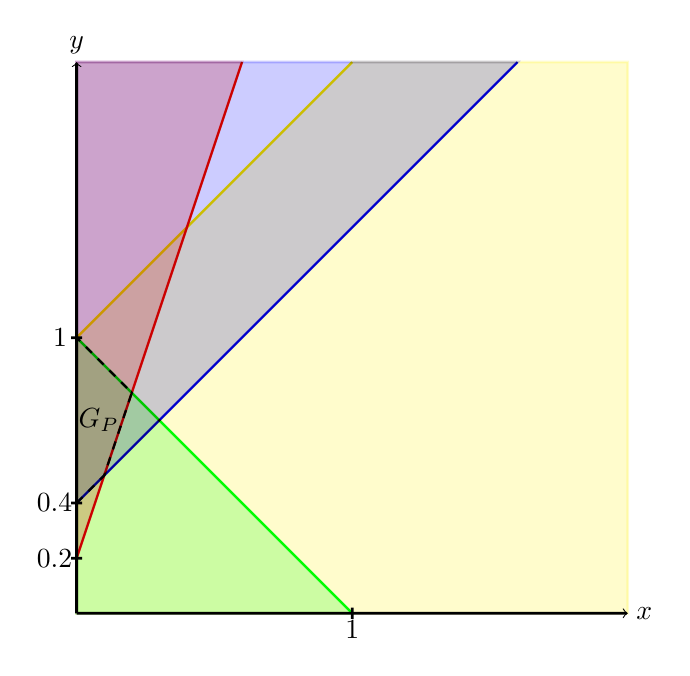
\begin{tikzpicture}[scale=0.7]
		\begin{scope}[transparency group]
		\begin{scope}[blend mode=multiply]
		\draw[->] (0,0) -- (10,0);
		\draw[->] (0,0) -- (0,10);
		\node at (10.3,0) (y) {$x$};
		\node at (0,10.3) (x) {$y$};
		
		\draw (-0.1,5) -- (0.1,5);
		\node at (-0.3,5) (1y) {1};
		\draw (-0.1,2) -- (0.1,2);
		\node at (-0.4,2) (0.4y) {0.4};
		\draw (-0.1,1) -- (0.1,1);
		\node at (-0.4,1) (0.4y) {0.2};
		\draw (5,-0.1) -- (5,0.1);
		\node at (5,-0.3) (1x) {1};
		
		\draw[yellow,thick] (0,5) -- (5,10);
		\draw[green,thick] (0,5) -- (5,0);
		\draw[blue,thick] (0,2) -- (8,10);
		\draw[red,thick] (0,1) -- (3,10);
		
		\draw[yellow, fill=yellow, opacity=0.2] (0,5) -- (5,10) -- (10,10) -- (10,0) -- (0,0) -- (0,5);
		\draw[green, fill=green, opacity=0.2] (0,5) -- (5,0) -- (0,0) -- (0,5);
		\draw[blue, fill=blue, opacity=0.2] (0,2) -- (8,10) -- (0,10) --(0,2);
		\draw[red, fill=red, opacity=0.2] (0,1) -- (3,10) -- (0,10) -- (0,1);
		
		\draw[dashed, thick, black] (0,2) -- (0.5,2.5) -- (1,4) -- (0,5) -- (0,2);
		\node at (0.4,3.5) (GP) {$G_P$};
		\end{scope}
		\end{scope}
		\end{tikzpicture}
	\end{center}
	Aus der graphischen Darstellung des zulässigen Bereiches und Parallelverschieben der Niveaulinie der Zielfunktion
	\begin{align}
		-2x_1+x_2 =c \notag
	\end{align}
	\begin{center}
		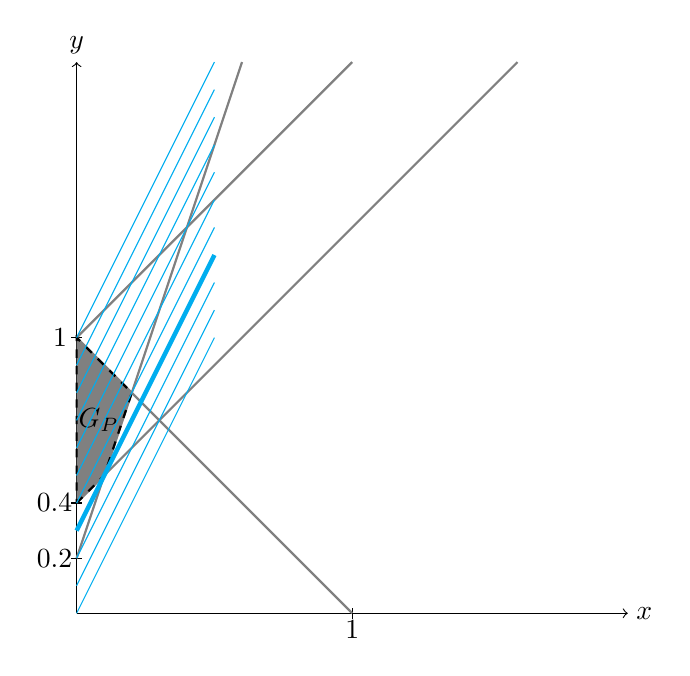
\begin{tikzpicture}[scale=0.7]
		\draw[->] (0,0) -- (10,0);
		\draw[->] (0,0) -- (0,10);
		\node at (10.3,0) (y) {$x$};
		\node at (0,10.3) (x) {$y$};
		
		\draw (-0.1,5) -- (0.1,5);
		\node at (-0.3,5) (1y) {1};
		\draw (-0.1,2) -- (0.1,2);
		\node at (-0.4,2) (0.4y) {0.4};
		\draw (-0.1,1) -- (0.1,1);
		\node at (-0.4,1) (0.4y) {0.2};
		\draw (5,-0.1) -- (5,0.1);
		\node at (5,-0.3) (1x) {1};
		
		\draw[gray,thick] (0,5) -- (5,10);
		\draw[gray,thick] (0,5) -- (5,0);
		\draw[gray,thick] (0,2) -- (8,10);
		\draw[gray,thick] (0,1) -- (3,10);
		
		\draw[dashed, thick, black, fill=gray] (0,2) -- (0.5,2.5) -- (1,4) -- (0,5) -- (0,2);
		\node at (0.4,3.5) (GP) {$G_P$};
		
		\draw[cyan] (0,5) -- (2.5,10);
		\draw[cyan] (0,4.5) -- (2.5,9.5);
		\draw[cyan] (0,4) -- (2.5,9);
		\draw[cyan] (0,3.5) -- (2.5,8.5);
		\draw[cyan] (0,3) -- (2.5,8);
		\draw[cyan] (0,2.5) -- (2.5,7.5);
		\draw[cyan] (0,2) -- (2.5,7);
		\draw[cyan, ultra thick] (0,1.5) -- (2.5,6.5);
		\draw[cyan] (0,1) -- (2.5,6);
		\draw[cyan] (0,0.5) -- (2.5,5.5);
		\draw[cyan] (0,0) -- (2.5,5);
		\end{tikzpicture}
	\end{center}
	erhält man das minimale $c$, bei dem die Niveaulinie und der zulässige Bereich noch den gemeinsamen Punkt $(x_1^\ast,x_2^\ast)=(0.1,0.5)$ haben und $c=0.3$. Zur Überführung der Optimierungsaufgabe in Standardform fügt man nicht-negative Schlupfvariablen $y_1,...,y_4$ hinzu:
	\begin{align}
		x_1-x_2+y_1+0.4 &= 0 \notag \\
		-x_1+x_2+y_2-1 &= 0 \notag \\
		3x_1-x_2+y_3+0.2 &= 0\notag \\
		x_1+x_2+y_4-1 &= 0\notag \\
		x_1,x_2 &\ge 0\notag \\
		y_1,y_2,y_3,y_4 &\ge 0 \notag
	\end{align}
	Eine andere gegebenenfalls erforderliche Umformung, um aus einer gegebenen linearen Optimierungsaufgabe deren Standardform zu erhalten, betrifft die Substitution von nicht vorzeichenbeschränkten Variablen, so kann $w\in\real$ etwa durch
	\begin{align}
		w = u-v\quad\text{mit}\quad u,v\ge 0\notag
	\end{align}
	ersetzt werden.
\end{example}
